% -----------------------------------------------------------------------------
\subsection{Geant4 Tasks Performance Analysis on Titan}
\label{ssec:panda_titan}

Currently, 20 instances of PanDA Broker are concurrently deployed on a total of
4 DTNs, 5 instances for each DTN. Each broker controls from 15 to 300 ATLAS
simulation jobs per submission, for a maximum total of 96,000 cores. Since
November 2015, the brokers have operated only in backfill mode, without a
defined time allocation, and running at the lowest priority on Titan.
Figure~\ref{core-hours-utilization} shows Titan core hours used by ATLAS from
September 2015 to March 2017. During that period, ATLAS consumed about XX
million Titan core hours. About XX million detector simulation jobs were
completed, and more than 132 million events processed. In February 2017, we
exceeded X million core hours per month and by March 2017 we ran at more than
X million core hours per month.

Figure~\ref{backfill-utilization} shows backfill utilization efficiency, defined
as a fraction of Titan’s total free resources that were utilized by ATLAS, for
the period from September 2015 to March 2017. Due to continuos improvements in
the system, the efficiency grew from less than 5\% to more than XX\%, reaching
XX\% in February 2017. At the peak, this corresponds to more than X\%
improvement in Titan’s overall utilization.

\mtnote{Add new diagram as discussed in F2F meeting at Rutgers.}

% -----------------------------------------------------------------------------
\subsection{PanDA Shared Library I/O Performance Impact at OLCF}

Athena, the ATLAS framework has a configuration and initialization stage. At
this stage, the running job is assembled  on the fly from a large number of
shared libraries.  Also, at this stage, every algorithm and service is being
configured, at run time, by a corresponding set of Python scripts, which
results in a large number of read operations accesses to small python scripts, with
many includes and imports Python calls.

When ATLAS was originally deployed at the OLCF, all shared libraries were
placed at the Spider 2 Lustre file system. However, it was quickly discovered
that the I/O pattern at the Athena stage was detrimental to the overall Spider
2 file system performance. Since Spider 2 is a center-wide file system and
shared by all OLCF resources and users, this resulted in lower overall
interactive and metadata performance at OLCF\@. As can be seen in
Listing~\ref{mdstrace} the metadata I/O activity for ATLAS exhibits a spike
corresponding to the beginning of the runs before tapering off.

\begin{minipage}{\linewidth}
\begin{lstlisting}[language=bash,frame=single,basicstyle=\ttfamily\tiny,caption=ATLAS metadata trace,label=mdstrace]
XK7 Application 9205593
      39012 RPCs from 300 of 300 nodes
        ~69291.96 per sec
          37851 LDLM_ENQUEUE RPCs    ~67229.83 per sec
                pmin 13us pavg 42us pmax 4983us
          611 LDLM_CANCEL RPCs    ~1085.24 per sec
                pmin 10us pavg 16us pmax 32us
          277 MDS_CLOSE RPCs    ~492.00 per sec
                pmin 15us pavg 20us pmax 38us
          154 MDS_READPAGE RPCs    ~273.53 per sec
                pmin 170us pavg 292us pmax 671us
          86 MDS_GETXATTR RPCs    ~152.75 per sec
                pmin 15us pavg 21us pmax 65us
          30 MDS_GETATTR RPCs    ~53.29 per sec
                pmin 16us pavg 20us pmax 27us
          3 MDS_REINT RPCs    ~5.33 per sec
                pmin 103us pavg 136us pmax 196us
          Overall times
                pmin 10us pavg 42us pmax 4983us

XK7 Application 9205355
      8698 RPCs from 62 of 62 nodes
        ~15449.13 per sec
          8445 LDLM_ENQUEUE RPCs    ~14999.76 per sec
                pmin 16us pavg 41us pmax 780us
          92 MDS_CLOSE RPCs    ~163.41 per sec
                pmin 15us pavg 23us pmax 52us
          55 MDS_READPAGE RPCs    ~97.69 per sec
                pmin 189us pavg 291us pmax 534us
          52 LDLM_CANCEL RPCs    ~92.36 per sec
                pmin 12us pavg 16us pmax 25us
          41 MDS_GETXATTR RPCs    ~72.82 per sec
                pmin 16us pavg 20us pmax 27us
          13 MDS_GETATTR RPCs    ~23.09 per sec
                pmin 16us pavg 21us pmax 38us
          Overall times
                pmin 12us pavg 42us pmax 780us

\end{lstlisting}
\end{minipage}

As this problem was identified, the OLCF staff has enabled read-only access to
certain NFS-exported directories from Titan compute nodes. This in turn allowed
the OLCF staff to install a software package from a Titan login node and have
it available read-only on a Titan compute node.

After moving the ATLAS release on Lustre to the NFS-exported read-only
directories, the metadata contention problem has resolved and a two orders of
magnitude metadata performance improvement (i.e., \~6,300 seconds on Lustre vs.\
\~1,500 seconds on NFS) has been observed for ATLAS\@.  Also, for both cases the
input file is placed on memory disk on a Titan compute nodes and for Lustre the
validation step took on average 1,320 seconds, while it was 40 seconds on NFS,
showing a three orders of magnitude performance improvement.

%Figure~\ref{fig:atlas-perf-improvement} shows the overall ATLAS performance
%improvement on Titan. The circled region illustrates the switch from Lustre to
%NFS-exported directory for hosting the ATLAS release.

%\begin{figure}[!htb]
%    \centering
%    \begin{tabular}{cc}
%        {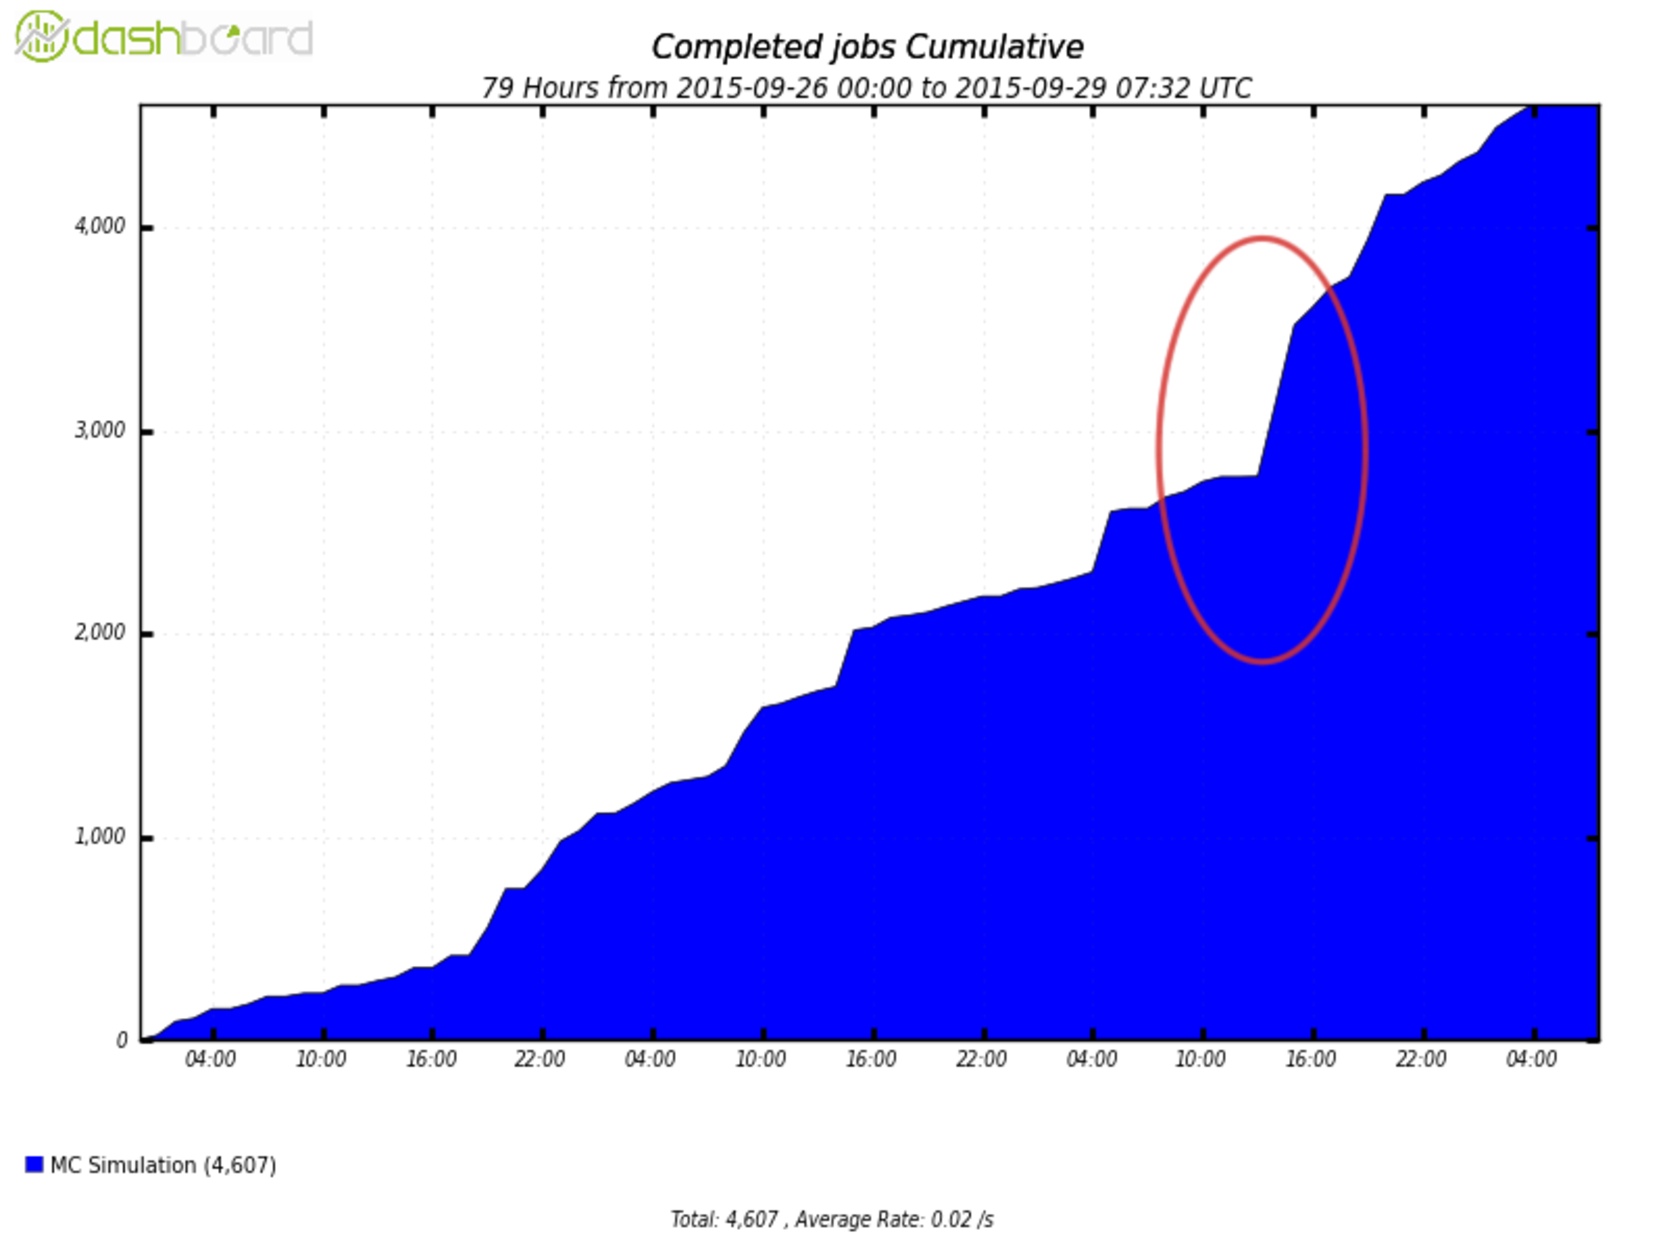
\includegraphics[width=0.48\textwidth]{figures/panda-completed-jobs-sw-move.pdf}}\\
%    \end{tabular}
%    \caption{ATLAS performance improvement on Titan. The circled region shows the switch from Lustre to NFS-exported directory for hosting the ATLAS release.}
%\label{fig:atlas-perf-improvement}
%\end{figure}


\subsection{PanDA I/O Impact at OLCF}

To better understand the I/O impact of ATLAS PanDA project on Titan
supercomputing environment we analyzed 1,175 jobs ran on the week of 10/25/2016,
for a total of 174 hours. Table~\ref{panda-olcf-stats} shows the overall
statistical breakdown of the observed file I/O impact of ATLAS at OLCF\@.
Figures~\ref{fig:atlas-titan-io-read} and~\ref{fig:atlas-titan-io-written} show
the file read and write I/O histograms for these 1,175 jobs, respectively.
Figures~\ref{fig:atlas-titan-file-open} and~\ref{fig:atlas-titan-file-close}
show the file $open()$ and $close()$ metadata load histograms of the same 1,175
ATLAS jobs, respectively.

As can be seen from Table~\ref{panda-olcf-stats}, the number of nodes used by
ATLAS jobs vary between 1 and 300, while the average is at 35. 75\% of the
ATLAS jobs consume less than 25 and 92\% consume less than or equal to 100
Titan compute nodes. During the 174 hours of data collection, we observed that
6.75 ATLAS jobs were executed on average per hour on Titan and ran for
1.74 hours on average.

ATLAS jobs issues a large number of file read operations, as can be seen in
Table~\ref{panda-olcf-stats}. The maximum amount read by any ATLAS job in
aggregate in this observed period was less than 250 GB and the maximum amount
written in aggregate was less than 75 GB\@. The average amount read per job is
20 GB and average amount written is 6 GB\@.

\begin{figure}[!htb]
    \centering
    \begin{tabular}{cc}
        {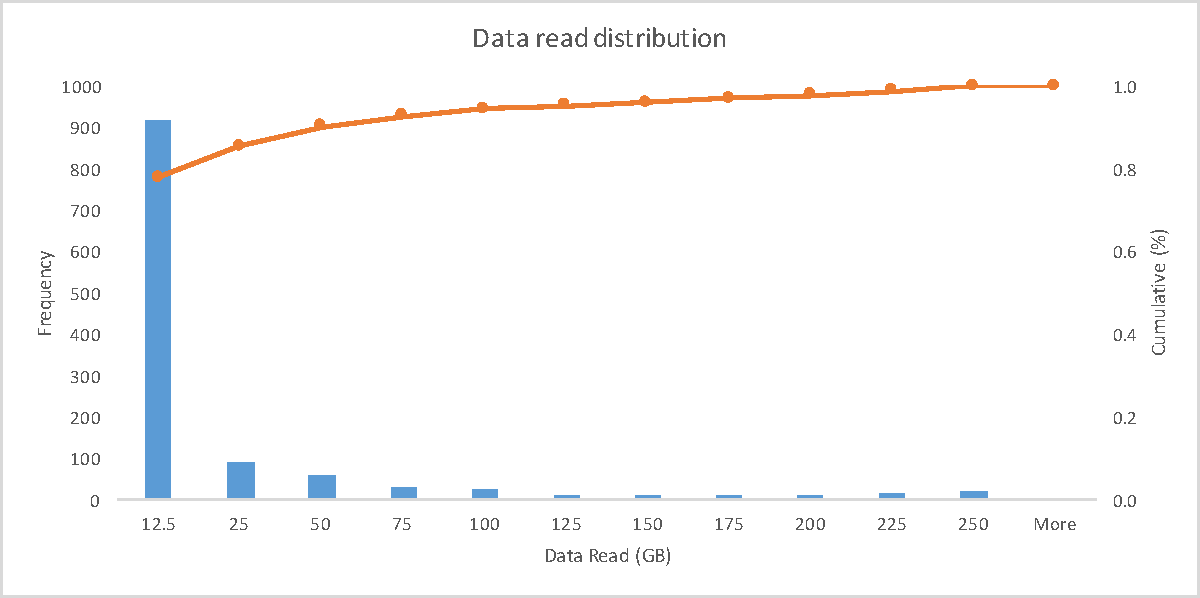
\includegraphics[width=0.48\textwidth]{figures/panda_data_read_finer_hist.pdf}}\\
    \end{tabular}
    \caption{ATLAS file read operation histogram on Titan for week of 10/25/16.}
\label{fig:atlas-titan-io-read}
\end{figure}



\begin{figure}[!htb]
    \centering
    \begin{tabular}{cc}
        {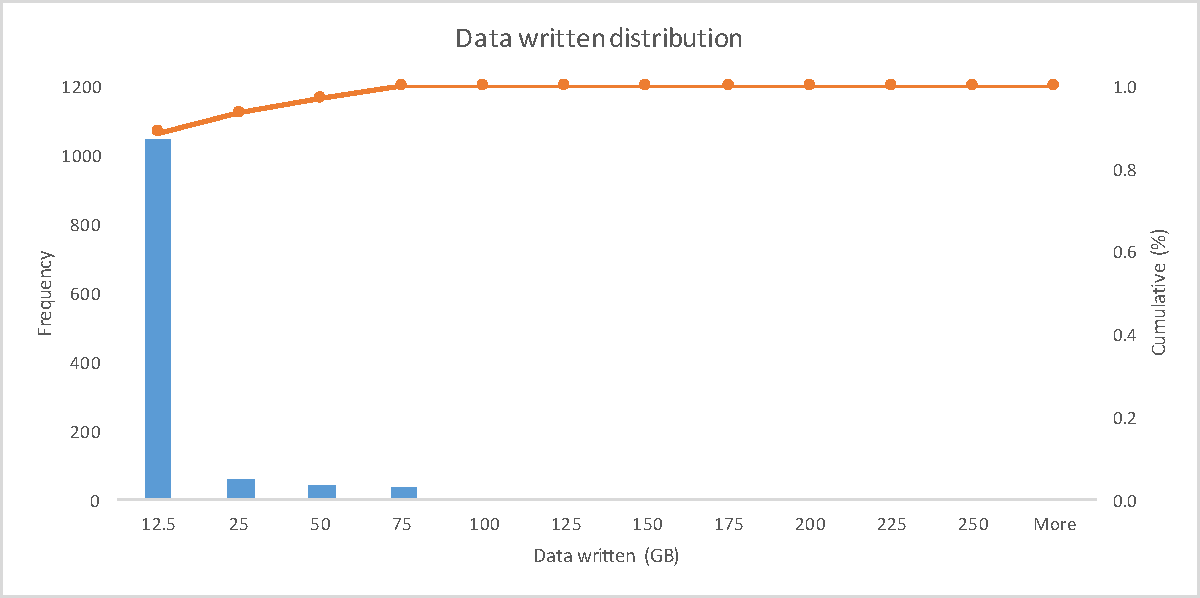
\includegraphics[width=0.48\textwidth]{figures/panda_data_written_finer_hist.pdf}}\\
    \end{tabular}
    \caption{ATLAS file write I/O histogram on Titan for week of 10/25/16.}
\label{fig:atlas-titan-io-written}
\end{figure}


Per job read and write file I/O statistics show an interesting pattern.
Table~\ref{panda-olcf-stats} indicates that the amount of data read per ATLAS
compute node on Titan is less than 400 MB on average, while the amount of data
written per node is less than 170 MB on average. This correlates with our
finding that ATLAS PanDA jobs are read heavy. However, as can be seen in
Table~\ref{panda-olcf-stats} and figures {fig:atlas-titan-io-read} and
{fig:atlas-titan-io-written}, the distribution between read and written amount
of data per job is quite different from one another. The read operation distribution
per job shows a long tail, ranging from 12.5 GB to 250 GB, while the written
amount of data has a very narrow distribution.

\begin{figure}[!htb]
    \centering
    \begin{tabular}{cc}
        {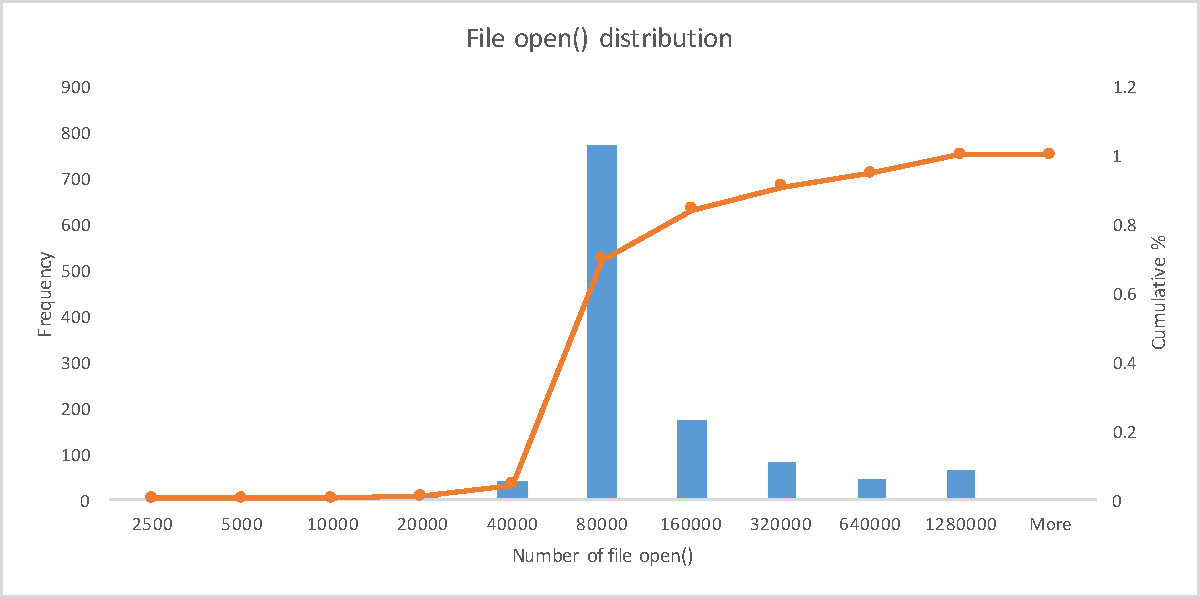
\includegraphics[width=0.48\textwidth]{figures/panda_file_open_hist.pdf}}\\
    \end{tabular}
    \caption{ATLAS file $open()$ histogram on Titan for week of 10/25/16.}
\label{fig:atlas-titan-file-open}
\end{figure}


\begin{figure}[!htb]
    \centering
    \begin{tabular}{cc}
        {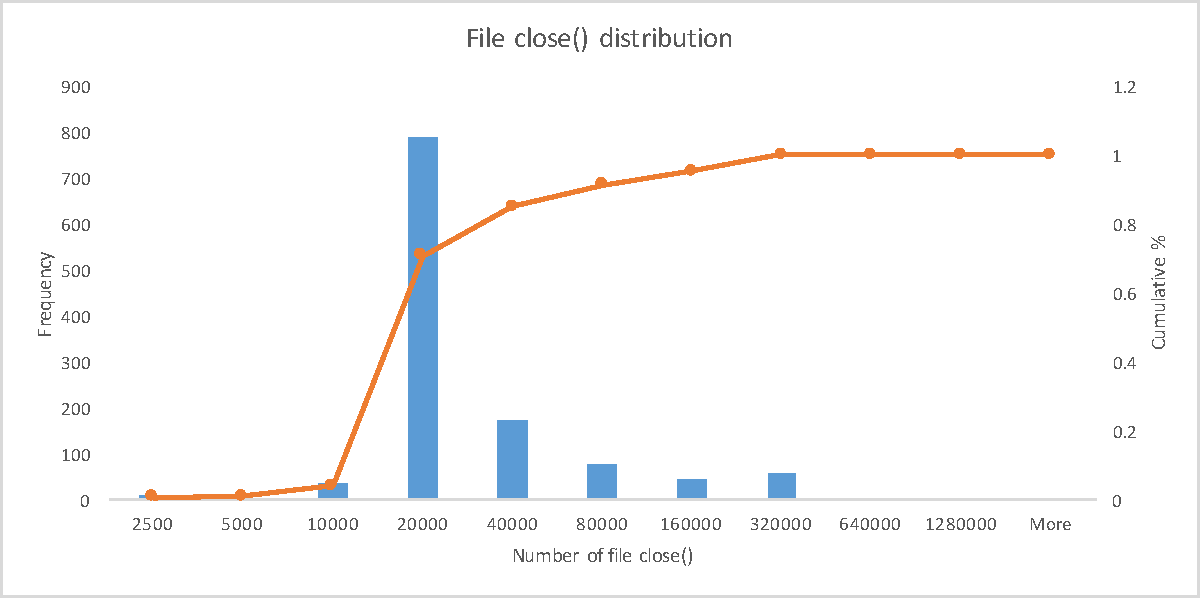
\includegraphics[width=0.48\textwidth]{figures/panda_file_close_hist.pdf}}\\
    \end{tabular}
    \caption{ATLAS file $close()$ histogram on Titan for week of 10/25/16.}
\label{fig:atlas-titan-file-close}
\end{figure}

On the metadata I/O breakdown, ATLAS PanDA jobs yield 23 file $open()$
operations and 5 file $close()$ operations per second. The file $open()$
operations listed here don't include the file $stat()$ operations. As can be
seen from figures~\ref{fig:atlas-titan-file-open}
and~\ref{fig:atlas-titan-file-close}, they exhibit similar distributions. The
maximum number of file $open()$ operations are around 170 on average and the
maximum number of file $close()$ operations are 39 on average per second per
job. The total number of file $open()$ operations is 172,089,760 for the
observed window of 174 hours, while the total number of file $close()$
operations stand at 40,132,992 for the total 1,175 ATLAS PanDA jobs in the same
observation window. The difference between these two values is puzzling and it
is under investigation at the time of writing this paper. One possible
explanation is that ATLAS PanDA jobs perhaps don't call a file $close()$
operation per every file $open()$ issued.



\begin{table*}[t]
\centering
\begin{tabular}{lllllllll}
 & Num. Nodes & Duration (s) & Read (GB) & Written (GB) & GB Read/nodes & GB Written/nodes & $open()$ & $close()$ \\
Min & 1 & 1,932 & 0.01 & 0.03 & 0.00037 & 0.02485 & 1,368 & 349 \\
Max & 300 & 7,452 & 241.06 & 71.71 & 0.81670 & 0.23903 & 1,260,185 & 294,908 \\
Average & 35.66 & 6,280.82 & 20.36 & 6.87 & 0.38354 & 0.16794 & 146,459.37 & 34,155.74 \\
Std. Dev. & 55.33 & 520.99 & 43.90 & 12.33 & 0.19379 & 0.03376 & 231,346.55 & 53,799.08
\end{tabular}
\caption{The Statistical breakdown of the I/O impact of 1,175 PanDA jobs executed at OLCF for the week of 10/25/16}
\label{panda-olcf-stats}
\end{table*}

Overall, based on our experiments with real-world jobs, it can be safely
concluded that the file and metadata I/O load of ATLAS PanDA project on the
OLCF Titan supercomputing environment and the Spider 2 file system is not
detrimental to the center operations and the overall impact is minimal, at the
current scale of the project.
